\documentclass[10pt,mathserif,t]{beamer}

\usepackage{graphicx,amsmath,amssymb,tikz,psfrag}
\usepackage{listings}
\usepackage{algorithmic}

\usepackage[natbib=true,style=authoryear,backend=bibtex,useprefix=true]{biblatex}
\setbeamercolor*{bibliography entry title}{fg=black}
\setbeamercolor*{bibliography entry location}{fg=black}
\setbeamercolor*{bibliography entry note}{fg=black}
\setbeamertemplate{bibliography item}{}
\renewcommand*{\bibfont}{\scriptsize}
\addbibresource{bibliography.bib}

\input defs.tex

%% formatting

\mode<presentation>
{
\usetheme{default}
}
\setbeamertemplate{navigation symbols}{}
\definecolor{UBCblue}{rgb}{0.04706, 0.13725, 0.26667} % UBC Blue (primary)
\usecolortheme[named=UBCblue]{structure}
\setbeamertemplate{itemize subitem}{--}
\setbeamertemplate{frametitle} {
	\begin{center}
	  {\large\bf \insertframetitle}
	\end{center}
}

\newcommand\footlineon{
  \setbeamertemplate{footline} {
    \begin{beamercolorbox}[ht=2.5ex,dp=1.125ex,leftskip=.8cm,rightskip=.6cm]{structure}
      \footnotesize \insertsection
      \hfill
      {\insertframenumber}
    \end{beamercolorbox}
    \vskip 0.45cm
  }
}
\footlineon

\AtBeginSection[] 
{ 
	\begin{frame}<beamer> 
		\frametitle{Outline} 
		\tableofcontents[currentsection,currentsubsection] 
	\end{frame} 
} 

%% begin presentation

\title{\large \bfseries Interpretable Machine Learning}

\date{}

\begin{document}
	
\newcommand{\code}[1]{\textcolor{magenta}{\texttt{#1}}}

\lstdefinestyle{pycode}{
	language=python,
	basicstyle=\ttfamily\color{magenta},
	commentstyle=\color{black}
}

\frame{
\thispagestyle{empty}
\titlepage
}

%----------------------------------------------------------------------------------------
%	PRESENTATION SLIDES
%----------------------------------------------------------------------------------------
\section{Foundations}

\begin{frame}[c]
\Huge{\centerline{Foundations}}
\end{frame}

%----------------------------------------------------------------------------------------

\begin{frame}\frametitle{Introduction \& Purpose}
	\begin{itemize}
		\item \textbf{Goal:} Ability to interpret complex "black box" models, deemed uninterpretable for decades.
		\bigskip 
		\item \textbf{Solution:} Some approaches that increase a complex model's transparency, accountability, and fairness are the following:
		\bigskip
		\begin{itemize}
			\item Decision tree surrogate models [\cite{dt_surrogate1}; \cite{dt_surrogate2}]
			\item Partial dependence plots [\cite{esl}]
			\item Individual conditional expectation (ICE) plots [\cite{ice_plots}]
			\item Random forest feature importance [\cite{esl}]
			\item Leave-one-covariate-out (LOCO) local feature importance [\cite{conformal_reg}]
			\item Local Interpretable Model-agnostic Explanations (LIME) [\cite{lime}]
			\item Shapley Explanations [\cite{shapley}; \cite{tree_shap}]
			\end{itemize}
	\end{itemize}
\end{frame}
%----------------------------------------------------------------------------------------

\begin{frame}\frametitle{Introduction \& Purpose}
	\begin{itemize}
		\item The following slides will detail the mathematics behind each of these approaches and techniques. 
	\end{itemize}
\end{frame}

%----------------------------------------------------------------------------------------

\begin{frame}\frametitle{Notation \& Preliminaries}
	\begin{itemize}
		\item \textbf{Spaces}.  
			\begin{itemize}
				\item The input features come from a set  $\mathcal{X}$ contained in a \textit{P}-dimensional input space (i.e. $\mathcal{X} \subset \mathbb{R}^P)$.  
				\item The output responses come from a set $\mathcal{Y}$ contained in a $C$-dimensional output space (i.e. $\mathcal{Y} \subset \mathbb{R}^C$).
			\end{itemize}	
			\bigskip	
		\item \textbf{Dataset}. A dataset $\mathbf{D}$ consists of $N$ tuples of observations:\\ $[(\mathbf{x}^{(0)},\mathbf{y}^{(0)}), (\mathbf{x}^{(1)},\mathbf{y}^{(1)}), \dots, (\mathbf{x}^{(N-1)},\mathbf{y}^{(N-1)})], \mathbf{x}^{(i)} \in \mathcal{X}, \mathbf{y}^{(i)} \in \mathcal{Y}$.\\
			\begin{itemize}
			\item The input data $\mathbf{X}$ is composed of the set of row vectors $\mathbf{x}^{(i)}$. 
				\begin{itemize}
					\item let $\mathcal{P}$ be the set of features  $\{X_0, X_1, \dots, X_{P-1}\}$, where $X_j = \left[x_{j}^{(0)}, x_{j}^{(1)}, \dots, x_{j}^{(N-1)} \right]^T$.
					\item then each $i$-th observation denoted as $\mathbf{x}^{(i)} = \left[x_0^{(i)}, x_1^{(i)}, \dots, x_{P-1}^{(i)} \right]$ is an instance of $\mathcal{P}$.
				\end{itemize}
		\end{itemize}
	\end{itemize}
\end{frame}
%----------------------------------------------------------------------------------------

\begin{frame}\frametitle{Preliminaries (Cont.)}
	\begin{itemize}
		\item \textbf{Learning Problem}. We want to discover some \textit{unknown target function} $f: \mathcal{X} \rightarrow \mathcal{Y}$ from our data $\mathbf{D}$, which we assume is identically and independently distributed (i.i.d).  To do so, we explore a \textit{hypothesis set} $\mathcal{H}$ and use a given learning algorithm $\mathcal{A}$ to find a function $g$ that we hope sufficiently approximates our target function: $\mathbf{D} \xrightarrow[]{\mathcal{A}} g \approx f$.  For a given training example $(\mathbf{x}, \mathbf{y})$ in $\mathbf{D}$, we hope that $g(\mathbf{x}) = \hat{\mathbf{y}} \approx \mathbf{y}$ and $g$ generalizes well for unseen observations.
	\end{itemize}
\end{frame}

%----------------------------------------------------------------------------------------

\begin{frame}\frametitle{Preliminaries (Cont.)}
	\begin{figure}[htb]
	\begin{center}
		\includegraphics[width=0.77\textwidth]{images/learning_problem.png}
		\caption{The learning problem. Adapted from \textbf{Learning From Data}.}
		\label{fig:learning_problem}
	\end{center}
	\end{figure}
\end{frame}

%----------------------------------------------------------------------------------------

\begin{frame}\frametitle{Preliminaries (Cont.)}
	\begin{itemize}
		\item \textbf{Explanation}. To justify the predictions of $g(\mathbf{x})$, we may resort to a number of techniques. Some techniques will be global in scope and simply seek to generate an interpretable approximation, $h$, for $g$ itself, such that $h(\mathbf{x}) \approx g(\mathbf{x}) = \hat{\mathbf{y}}(\mathbf{x})$. Other techniques will be more local in scope and attempt to rank local contributions for each feature $X_j \in \mathcal{P}$ for some observation $\mathbf{x}^{(i)}$; this can create reason codes for $g(\mathbf{x}^{(i)})$. Local contributions are often estimated by evaluating the product of a learned parameter $\beta_j$ in $g$ with a corresponding observed feature value $x_j^{(i)}$ (i.e. $\beta_jx_j^{(i)}$), or by seeking to remove the contribution of some $X_j$ in a prediction, $g(\mathbf{x}_{(-j)}^{(i)})$.
	\end{itemize}
\end{frame}





\section{Interpretability}

\begin{frame}[c]
\Huge{\centerline{Interpretability}}
\end{frame}
%----------------------------------------------------------------------------------------

\begin{frame}\frametitle{Model Complexity}

	\begin{itemize}
		\item The more complex a function, the more difficult it is to explain. Simple functions can be used to explain more complex functions, however not all explanatory techniques are a good match for all types of models. 
		\bigskip
		\item When interpreting a complex model, it is important to verify that your interpretation techniques:
		\begin{itemize}
			\item are appropriate for the response function complexity of the model.
			\item are appropriate for global and local interpretation.
			\item make sense given real-world context (aka match domain expertise).
			\item provide explanations that match the explanations of other interpretation techniques.
		\end{itemize}
		\end{itemize}
\end{frame}

%----------------------------------------------------------------------------------------

\begin{frame}\frametitle{Model Complexity (Cont.)}	
	\begin{itemize}
		\item \textbf{7} different techniques are presented to help interpret the results of your complex model. These techniques should be reviewed individually and within the general context of all other techniques. Depending on the relationship between your input training data and your target, certain interpretation techniques will be more reliable than others. These 7 techniques fall into two categories \textbf{model-agnostic} and \textbf{model-specific}, explained in the next section.
		\bigskip
		\item The \textbf{7} techniques were chosen based on the essential questions they could answer about a complex model, including but not limited to:
		\begin{itemize}
			\item how features are handled
			\item how interactions are handled
			\item the impact of individual features
			\item how to create reason codes
		\end{itemize}
	\end{itemize}
\end{frame}


%----------------------------------------------------------------------------------------

\begin{frame}\frametitle{Specific Interpretability Techniques}

	\begin{itemize}
		\item \textbf{Model Agnostic:} Techniques to interpret the inner workings of any model. Requires surrogate models (detailed in next section), which can degrade the interpretation's quality. Since there is no guarantee that a surrogate model reflects the decisions of a complex model, it is important to verify how well a surrogate model fits the results of the complex model before using it as a method of interpretation.
		\begin{itemize} 
			\item Decision Tree \textbf{Surrogate} Models
			\item Partial Dependence Plots
			\item Individual Conditional Expectation Plots
			\item LOCO
		\end{itemize} 
		\bigskip
		\item \textbf{Model Specific:} Techniques that are attributed to and require specific models.
		\begin{itemize}
			\item Random Forest or Gradient Boosting Variable Importance.
			\item Shapley: Tree Shap Implementation.
			\item Local Interpretable Model-agnostic Explanations (LIME).
		\end{itemize} 
	\end{itemize}
\end{frame}

\section{Surrogate Models}

\begin{frame}[c]
\Huge{\centerline{Surrogate Models}}
\end{frame}

%----------------------------------------------------------------------------------------

\begin{frame}\frametitle{Surrogate Models}
	\begin{itemize}
	        \item A \textit{surrogate model} is a data mining and engineering technique in which a simple model is used to explain another complex model.
		\item Given our learned function $g$ and set of predictions, $g(\mathbf{X}) = \hat{\mathbf{Y}}$, we can train a surrogate model $h$:
			
			\begin{equation}
			\begin{aligned}
				 \mathbf{X},\hat{\mathbf{Y}} \xrightarrow{\mathcal{A}_{\text{surrogate}}} h\
			\end{aligned}
			\end{equation}
		\item Ideally $h(\mathbf{X}) \approx g(\mathbf{X})$, however there exist few guarantees that $h(\mathbf{X})$ accurately represents $g$.
		\item To preserve interpretability, the hypothesis set for $h$ is often restricted to linear models or decision trees.
	\end{itemize}
\end{frame}

%----------------------------------------------------------------------------------------

\begin{frame}\frametitle{Surrogate Models (Cont.)}
	\begin{itemize}
	        \item While any model can act as a surrogate model, surrogate models are chosen because they are easy for a human to interpret and explain. Surrogate models enhance transparency by providing:
	        \bigskip
	        \begin{itemize}
	        \item Specific insights into the mechanism and results of a complex model.
	        \item Global or local interpretations of a complex model.
	        \item Visualizations that are easy to understand and compare.
	        \end{itemize}
	        \bigskip
	        \item Surrogate models are limited to linear models, decision trees, and random forests.
	
	\end{itemize}
\end{frame}

%----------------------------------------------------------------------------------------


\section{Decision Tree Surrogate Model}

\begin{frame}[c]
\Huge{\centerline{Decision Tree Surrogate Model}}
\end{frame}

%----------------------------------------------------------------------------------------

\begin{frame}\frametitle{Decision Tree Surrogate Model}
	\begin{itemize}
		\item Given our learned function $g$ and set of predictions, $g(\mathbf{X}) = \hat{\mathbf{Y}}$, we can train a decision tree surrogate model:
			\begin{equation}
			\begin{aligned}
				h_{\text{tree}}: \mathbf{X},\hat{\mathbf{Y}} \xrightarrow{\mathcal{A}_{\text{surrogate}}} h_{\text{tree}}
			\end{aligned}
			\end{equation}

		\item The decision tree surrogate model displays an approximate flow chart of $g$'s decision making process to increase model transparency.
		\item It also shows likely important features and the most important interactions in $g$. 
		
	\end{itemize}
\end{frame}

%----------------------------------------------------------------------------------------

\section{Partial Dependence Plots}

\begin{frame}[c]
\Huge{\centerline{Partial Dependence Plots}}
\end{frame}
%----------------------------------------------------------------------------------------

\begin{frame}\frametitle{Review of Marginal Expectation}
	\begin{itemize}
		\item Recall that in a $P$-dimensional feature space, we can consider a single feature $X_j \in \mathcal{P}$ and its complement set $\mathcal{P}_{(-j)}$ (where $\{X_j\} \cup \mathcal{P}_{(-j)} = \mathcal{P}$). 
		\item To describe the partial dependence $g(\mathbf{X})$ on $X_j$, we go through the following enumerated explanation:
		\begin{enumerate}
			\item Expected value is $\mathbb{E}[g\mathbf(X)] = \displaystyle\sum_{i = 0}^{N-1}g(x^{(i)})p(x^{(i)})$.
			\item  Let $g(\mathbf{X}) = g(X_j, X_{(-j)})$ and set $X_j = [x_{j}^{0}, \dots, x_{j}^{P-1}]^T)$. 
			\item Then the marginal expectation over $X_{(-j)}$ is $\mathbb{E}_{X_{(-j)}}\left[g(X_j, X_{(-j)})\right] =  \displaystyle\sum_{i = 0}^{N-1} g(X_j, X_{(-j)}) p(x^{(i)})$.
			\item Given that  $\displaystyle\sum_{i = 0}^{N-1} p(x^{(i)}) = 1$, and equal probabilities, $p(x^{(i)}) = \frac{1}{N}$.
			\item Thus $\mathbb{E}_{X_{(-j)}}\left[g(X_j, X_{(-j)})\right] = \displaystyle\frac{1}{N}\sum_{i = 0}^{N-1}g(x_j, \mathbf{x}_{(-j)}^{(i)})$.
		\end{enumerate}
	\end{itemize}
\end{frame}

%----------------------------------------------------------------------------------------

\begin{frame}\frametitle{Partial Dependence Plots (Cont.)}
	\begin{itemize}
	\item The partial dependence of a given feature $X_j$ is the average of the response function $g$, where all the components of $X_j$ are set to $x_j$ $(X_j= [x_j^{(0)}, \dots, x_j^{(N-1)}]^T)$, and all other feature vectors of the complement set $\mathbf{x}_{(-j)}^{(i)}$ are left as the original dataset specified.
	\item Thus, the \textit{one-dimensional partial dependence} of a function $g$ on  $X_j$ is the marginal expectation:
			\begin{equation}\label{eq:pd1}
			\begin{aligned}
				\text{PD}(X_j, g) &= \mathbb{E}_{X_{(-j)}}\left[g(X_j, X_{(-j)})\right]\\
			&= \frac{1}{N}\sum_{i = 0}^{N-1}g(x_j, \mathbf{x}_{(-j)}^{(i)})
		\end{aligned}
		\end{equation}
	\end{itemize}
\end{frame}

%----------------------------------------------------------------------------------------


\begin{frame}\frametitle{Partial Dependence Plots (Cont.)}		
	\begin{itemize}
		\item Partial dependence plots show the partial dependence as a function of \textit{specific values} of our feature subset.
		\item The plots show how machine-learned response functions change based on the values of an input feature of interest, while taking nonlinearity into consideration and averaging out the effects of all other input features.
		\item Partial dependence plots enable increased transparency in $g$ and enable the ability to validate and debug $g$ by comparing a feature's average predictions across its domain to known standards and reasonable expectations. 
	\end{itemize}
\end{frame}

%----------------------------------------------------------------------------------------

\begin{frame}
\frametitle{Conceptual Example}
\begin{figure}
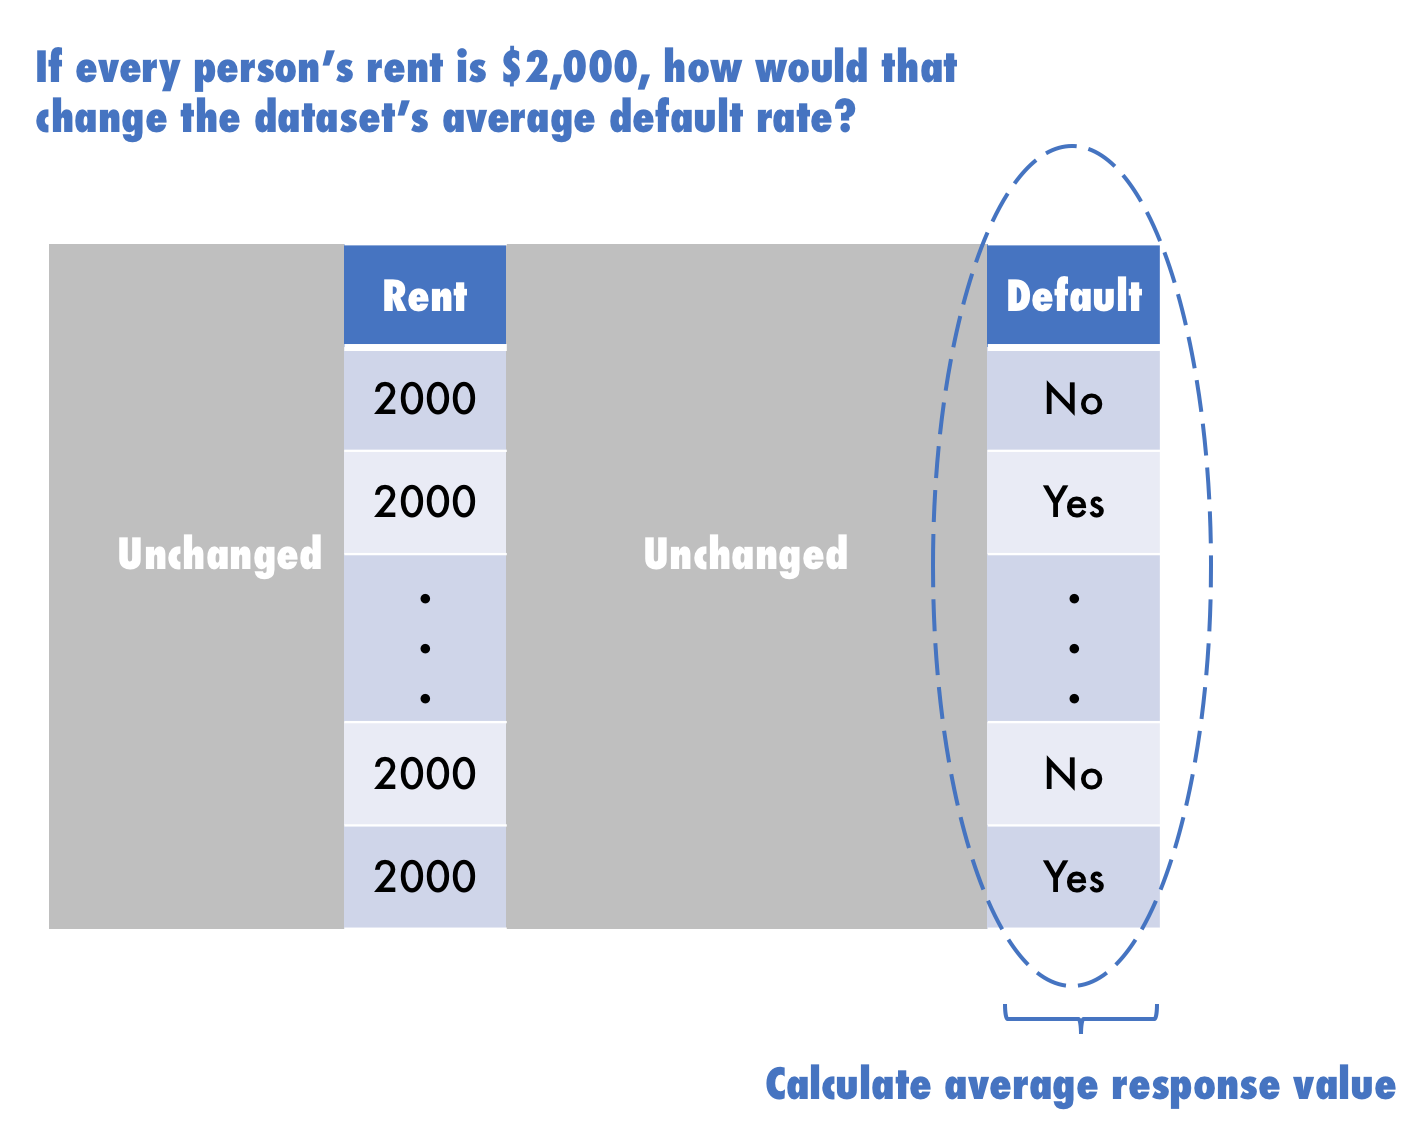
\includegraphics[scale=0.25]{images/pdp_image.png}
\caption{We want to predict whether someone will default on their monthly utility bill. The image shows one feature that we fixed ($Rent=2000$), keeping the rest unchanged, to see its impact on the dataset's average default rate.}
\end{figure}
\end{frame}
\section{Individual Conditional Expectation}

\begin{frame}[c]
\Huge{\centerline{Individual Conditional Expectation}}
\end{frame}

%----------------------------------------------------------------------------------------

\begin{frame}\frametitle{Individual Conditional Expectation}
	\begin{itemize}
		\item Individual conditional expectation (ICE) plots can create localized explanations for a single observation of data using the same basic ideas as partial dependence plots.
		\item ICE is a type of nonlinear sensitivity analysis in which a model's predictions for a single observation are measured while a feature of interest is varied over its domain.
		\item To create an ICE plot for a row of interest $x^{(i)}$ and a feature of interest $x_j^{(i)}$, we vary $x_j^{(i)}$ within the range of the feature's original domain, and call a single such value $x_{j,q}$ (where $q$ specifies an index within the domain):\\
		\bigskip
		 $\text{Specifically, we plot }g(x_{j,q}, \mathbf{x}_{(-j)}^{(i)}) \text{ versus } x_{j,q} \text{ for each fixed }\mathbf{x}_{(-j)}^{(i)}.$
	\end{itemize}
\end{frame}

%----------------------------------------------------------------------------------------
\section{Feature Importance}

\begin{frame}[c]
\Huge{\centerline{Feature Importance}}
\end{frame}


%----------------------------------------------------------------------------------------
\begin{frame}\frametitle{Feature Importance}

	\begin{itemize}			
		\item Feature Importance ($FI$) measures the effect that a feature has on the predictions of a model.  
		\item Unlike regression parameters, it is often unsigned and typically not directly related to the numerical predictions of the model.
	\end{itemize}
\end{frame}
%----------------------------------------------------------------------------------------

\begin{frame}\frametitle{Feature Importance}
	\begin{itemize}			
		\item \textbf{Global Importance}
			\begin{itemize} 
				\item measures the overall impact of an input feature on a model's predictions while taking nonlinearity and interactions into consideration.
				\item values give an indication of the magnitude of a feature's contribution to model predictions for all observations.		
			\end{itemize}
			\bigskip
		\item \textbf{Local Importance}
			\begin{itemize} 
				\item describes how the combination of the learned model rules or parameters and an individual observation's attributes affect a model's prediction for that observation while taking nonlinearity and interactions into effect. 
	\end{itemize}	
	\end{itemize}
\end{frame}

%----------------------------------------------------------------------------------------

\begin{frame}\frametitle{Random Forest Feature Importance }
To get the Global Feature Importance of a model on the original features, train a random forest model $h_{\text{RF}}$ with some target outcome.
		\begin{equation}
                            \begin{aligned}\label{eq:rf}
                            h_{\text{RF}}(\mathbf{x}^{(i)}) &= \frac{1}{B}\sum_{b=1}^B h_{\text{tree},b}\left(\mathbf{x}^{(i)}; \Theta_b\right)
                            \end{aligned}
		\end{equation}
		$B:$ number of decision trees \newline
		 $\Theta_b:$ set of splitting rules for each tree $h_{\text{tree},b}$  \newline
\end{frame}
%----------------------------------------------------------------------------------------


\begin{frame}\frametitle{Random Forest Feature Importance (cont.)}         
	\begin{itemize}
	\item At each split in each tree $h_{\text{tree},b}$, the improvement in the split-criterion is the importance measure attributed to the splitting feature, $X_{j}$. Specifically, the improvement is the difference between the squared error, $SE$, of the parent node $pn$ and the child nodes $cn$ at a given split. The importance measure is accumulated over all trees separately for each feature.
		\end{itemize}
\end{frame}

%----------------------------------------------------------------------------------------

\begin{frame}\frametitle{Random Forest Feature Importance (cont.)}         
	\begin{itemize}
	\item H2O splits a node to reduce the response variance in that node. 
	\item Then $SE$ is calculated by assuming an unbiased estimator (i.e. the mean squared error $MSE$ is equal to the variance $VAR$). Given that $SE=MSE\times{N}$, Then $SE=MSE\times{N}=VAR\times{N}$.
		\end{itemize}
		\begin{equation}
		 \begin{aligned}\label{eq:rf1}
                           VAR&=\frac{1}{N}\sum_{i=0}^{N-1}(y^{(i)}-\bar{y})^2\\
                           VAR\times{N}&=\left[\frac{1}{N}\times  \sum_{i=0}^{N-1}(y^{(i)})^2 -N\times{(\bar{y})^2} \right] \times N\\
                           &= \left[ \sum_{i=0}^{N-1}(\frac{(y^{(i)})^2}{N}) - \bar{y}^2 \right ]\times N=SE\\        
                 \end{aligned}
		\end{equation}     
\end{frame}


%----------------------------------------------------------------------------------------
%\begin{frame}\frametitle{Random Forest Feature Importance (cont.)}         
%A more generic form for calculating the $SE$ is also given below:
%
%		 \begin{equation}
%           	 \begin{aligned}
%				&SE_n=\sum_{i=1}^{N_{n}}w_i(y_i - \bar{y}_{n})^2\\
%				&\bar{y}_{n}=\frac{1}{N_{n}}\sum_{i=1}^{N_{n}}w_i y_i\\
%           	 \end{aligned}
%           	 \end{equation}
%        $SE_n$: the squared error for a given node.\\
%        $N_n$: the number of row-observations for a given node.\\
%	$n$: the index of each node. \\
%	$\bar{y}_n$: average predicted value for a given node.\\
%\end{frame}
%

%----------------------------------------------------------------------------------------


\begin{frame}\frametitle{Random Forest Feature Importance (cont.)}         
	\begin{itemize}
	\item at each split in each tree $h_{\text{tree},b}$, the improvement in the split-criterion is the importance measure attributed to the splitting feature, $X_{j}$. Specifically, the improvement is the difference between the squared error, $SE$, of the parent node $pn$ and the child nodes $cn$ at a given split. The importance measure is accumulated over all trees separately for each feature.
	\end{itemize}
		 \begin{equation}
		 \begin{aligned}\label{eq:rf1}
                            FI(X_{j})= \sum_{b=1}^B \sum_{tl=1}^{TD_{b}} \kappa \times SE_{tl}\\
                            \text{where } \kappa=\kappa(X_{j,tl})=\begin{cases}
                            1 & \text{if $X_{j,tl}=X_{j}$}\\
                            0 & \text{otherwise}
                            \end{cases}\\
                            SE_{tl}=SE_{pn}-SE_{cn}\\
                 \end{aligned}
		\end{equation}
		\bigskip

\hspace{3cm}$SE_{tl}$: Squared Error at tree level $tl$ \\
\hspace{3cm}$TD_{b}$: Max tree depth of each $b$ \\		
\hspace{3cm}$tl$: tree level \\
                         
\end{frame}

%----------------------------------------------------------------------------------------

\begin{frame}\frametitle{Random Forest Feature Importance }
	\begin{itemize}
		\item The aggregated feature importance values are then scaled between 0 and 1, such that the most important feature has an importance value of 1. \newline
		
		Let $m=\max\limits_{0 \leq l \leq P-1}FI(X_{l})$, $l=\text{index of feature } X_{l}$,\\
		then
	\begin{equation}
                          AF(X_{j}) = \frac{FI(X_{j})}{m}
	\end{equation}
	Where $AF(X_{j})$ is the aggregated feature importance.
	\end{itemize}
\end{frame}

\section{Leave One Covariate Out}

\begin{frame}[c]
\Huge{\centerline{Leave One Covariate Out}}
\end{frame}

%----------------------------------------------------------------------------------------
\begin{frame}\frametitle{Leave One Covariate Out}
	\begin{itemize}		
			\item Leave-one-covariate-out (LOCO) provides the feature importance values at a per-observation level (i.e. what is the feature importance of $X_j$ for observation $\mathbf{x}^{(i)}$).
			\bigskip
			\item LOCO is calculated by subtracting a model's prediction, $g(\mathbf{x}^{(i)})$, for a row-observation with all its features, from that model's prediction for the same row \textit{without} the input feature $X_j$ of interest. 	
		\begin{equation}
                           \begin{aligned}\label{eq:rf}
                            g(\mathbf{x}_{(-j)}^{(i)}) - g(\mathbf{x}^{(i)}),
                            \end{aligned}
		\end{equation}
where $\mathbf{x}_{(-j)}^{(i)} \in \mathcal{P}_{(-j)}$, given that $\mathcal{P}_{(-j)}$ is the complement set to $\{X_j\} \in \mathcal{P}$ (i.e $\{X_j\} \cup \mathcal{P}_{(-j)} = \mathcal{P}$).
	\end{itemize}
\end{frame}
%----------------------------------------------------------------------------------------






%-------------------------------------------------------------------------------
\section{Local Interpretable Model-agnostic Explanations (LIME)}
\begin{frame}[c]
\Huge{\centerline{LIME}}
\end{frame}
%-------------------------------------------------------------------------------
\begin{frame}
	\cite{lime} defines LIME for some observation $\mathbf{x} \in \mathcal{X}$:

	\begin{equation}
	\begin{aligned}
	\underset{h \in \mathcal{H}}{\arg\max}\:\mathcal{L}(g, h, \pi_{\mathbf{X}}) + \Omega(h)
	\end{aligned}
	\end{equation}

	Here $g$ is the function to be explained, $h$ is an interpretable surrogate model of $g$, often a linear model $h_{GLM}$, $\pi_{\mathbf{X}}$ is a weighting function over the domain of $g$, and $\Omega(h)$ limits the complexity of $h$.

	\vspace{5pt}

	Typically, $h_{GLM}$ is constructed such that

	\begin{equation}
	\begin{aligned}
	\mathbf{X}^{(*)}, g({X}^{(*)}) \xrightarrow{\mathcal{A}_{\text{surrogate}}} h_{\text{GLM}}
	\end{aligned}
	\end{equation}

	where $\mathbf{X}^{(*)}$ is a generated sample, $\pi_{\mathbf{X}}$ weighs $\mathbf{X}^{(*)}$ samples by their Euclidean similarity to $\mathbf{x}$, local feature importance is estimated using $\beta_j x_j$, and $L_1$ regularization is used to induce a simplified, sparse $h_{GLM}$. 
\end{frame}		

\begin{frame}\frametitle{LIME (Cont.)}
	\begin{itemize}
		
		\item LIME is ideal for creating highly interpretable explanations for non-decision tree models and for neural network models trained on unstructured data, e.g. deep learning models.
		
		\item Use regression fit measures to assess the trustworthiness of LIME explanations.
		
		\item Local feature importance values are offsets from a local intercept.
		
		\begin{itemize}
			
			\item Note that the intercept in LIME can account for the most important local phenomena.
			
			\item Generated LIME samples can contain large proportions of out-of-range data that can lead to unrealistic intercept values. 
			
		\end{itemize}
		
	\end{itemize}
\end{frame}

\begin{frame}\frametitle{LIME (Cont.)}
	\begin{itemize}
		
		\item To increase the trustworthiness of LIME explanations, try LIME on discretized input features and on manually constructed interactions.
		
		\item Use cross-validation to construct standard deviations or even confidence intervals for local feature importance values.
		
		\item LIME can fail, particularly in the presence of extreme nonlinearity or high-degree interactions.
		
	\end{itemize}
\end{frame}
\section{Shapley Feature Importance}

\begin{frame}[c]
\Huge{\centerline{Shapley Feature Importance}}
\end{frame}

%----------------------------------------------------------------------------------------

\begin{frame}\frametitle{Overview of SHAP: SHapley Additive exPlanations}

	\begin{itemize}
		\item \textbf{What:} SHAP values provide feature importance for a complex model, through numeric values that are easy for humans to understand. 
		\bigskip
		\item \textbf{Why:} SHAP is a unified framework that reveals the relationship between other published interpretability techniques [citations needed], as well as solutions to these techniques that are easier to interpret and satisfy the SHAP properties. 
		\bigskip
		\item\textbf{Examples:}  Interpretability methods that fall under the SHAP framework. \textit{Shapley Feature Importances} explicitly apply SHAP framework and satisfy its constraints, while \textit{LOCO} and \textit{Feature Importance} fall under the SHAP framework but are not designed to satisfy the SHAP Properties. 
	\end{itemize}
\end{frame}
%----------------------------------------------------------------------------------------

\begin{frame}\frametitle{SHAP: SHapley Additive exPlanations (Cont.)}

The following slides summarize and explain the work found in [\cite{shapley}].

\end{frame}
%----------------------------------------------------------------------------------------

\begin{frame}\frametitle{Explanation Models}

	\begin{itemize}
	\item \textbf{Explanation models:} a form of surrogate models, explanation models $h$ are designed to provide an interpretable approximation of a complex model. 
	\bigskip
	\item  \textbf{Simplified inputs:} a binary vector $\mathbf{x'}$, of interpretable values, that maps to a given training observation $\mathbf{x}$, through a mapping function $M_\mathbf{x}$ specific to $\mathbf{x}$, such that $\mathbf{x} = M_\mathbf{x}(\mathbf{x'})$.  
	\bigskip
	\item  \textbf{Local methods:} are techniques to explain a model's prediction for a specific observation, as oppose to observations in general.  When a local method works well, $h(\mathbf{z'}) \approx g(M_\mathbf{x}(\mathbf{z'}))$ whenever $\mathbf{z'} \approx \mathbf{x'}$.
	\end{itemize}
	
\end{frame}

%----------------------------------------------------------------------------------------

\begin{frame}\frametitle{Additive Feature Attribution Methods}
Additive feature attribution methods sum up the feature attributions of an observation  $\mathbf{x}$ to approximate and thereby explain the prediction $g(\mathbf{x})$ corresponding to that observation. 
	\bigskip
	\begin{itemize}
	\item  \textbf{Definition 1}  additive feature attribution methods use an explanation model that is a linear function of binary variables:
	\end{itemize}

	\begin{equation}
	\begin{aligned}		
		h(\mathbf{z'})= \phi_0 + \sum_{j=1}^P \phi_j z'_j,
	\end{aligned}
	\end{equation}
	
	$\phi_j$: each feature's attributed impact, where $\phi_j \in \mathbb{R}$.\\
	$P$: the number of predictors. \\
	$\mathbf{z'}$: the binary vector where $\mathbf{z'} \in \{0,1\}^P$.
	
\end{frame}

%----------------------------------------------------------------------------------------

\begin{frame}\frametitle{Review of Cooperative Game Theory's Shapley Number}
\begin{itemize}
	\item \textbf{Cooperative Games:} a game in which players benefit from teaming up rather than playing independently. 
	\bigskip
	\item \textbf{The Shapley Number:} a numeric value that determines how much a player should gain or lose, given the number of players and the value attributed to each if they were to play independently. 	\begin{itemize}
		\bigskip
		\item the Shapley Number is easy to calculate when there only a few players: it's the average value of all possible combinations for each player. 
	\end{itemize}
\end{itemize}
\end{frame}

%----------------------------------------------------------------------------------------

\begin{frame}\frametitle{Shapley Number Axioms}
The Shapley Number calculation is based on the following three axioms:
\begin{itemize}
	\bigskip
	\item \textbf{Efficiency}: the sum of the amounts attributed to each player must equal the total amount attributed to the players when they play together.
	\bigskip
	\item \textbf{Symmetry}: changing the names of players doesn't affect the attributed importance of each player.
	\bigskip
	\item \textbf{Monotonicity:} If the total value of a game increases the value attributed to each player will not decrease. This axiom includes the linearity axiom - the sum of players playing individually has to equal the sum of them playing together - and the null effect axiom - players that don't participate don't contribute to the game. 
\end{itemize}

\end{frame}

%----------------------------------------------------------------------------------------

\begin{frame}\frametitle{Game Theory Axiom Applied to Machine Learning}
The previous Shapley Number axioms can be applied as constraints to solve a SHAP explanation model. Below are the SHAP properties and their mapping to the Shapley axioms.
	\bigskip
\begin{itemize}
	\item Local Accuracy $\sim$ Efficiency Axiom
	\bigskip
	\item Missingness $\sim$ Null Effect Axiom - adapted to handle missing data
	\bigskip
	\item Consistency  $\sim$ Monotonicity Axiom

\end{itemize}


\end{frame}

%----------------------------------------------------------------------------------------

\begin{frame}\frametitle{Local Accuracy Property}
To satisfy the local accuracy property, an explanation model $h$ should return the same prediction as the complex model $g$, given a simplified input $\mathbf{x'}$ that maps back to $\mathbf{x}$ via the mapping function $M_\mathbf{x}$. Specifically, 

	\begin{equation}
	\begin{aligned}		
		&\text{if } \mathbf{x} = M_\mathbf{x}(\mathbf{x'}), \phi_0 = g(M_\mathbf{x}(\mathbf{0})),\\
		&\text{and } h(\mathbf{x'})= \phi_0 + \sum_{j=1}^P \phi_j x'_j,\\
		&\text{then } g(\mathbf{x}) = g(M_\mathbf{x}(\mathbf{x'})) = h(\mathbf{x'}).
	\end{aligned}
	\end{equation}


\end{frame}

%----------------------------------------------------------------------------------------

\begin{frame}\frametitle{Missingness Property}
If a feature value is missing during training, that implies it shouldn't have an attributed effect value. Remember that $x_j' = 0$ means the original input value $x_j$ is not present. 
 
	\begin{equation}
	\begin{aligned}	
		x_j' = 0 \implies \phi_j = 0
	\end{aligned}
	\end{equation}
	
\end{frame}

%----------------------------------------------------------------------------------------

\begin{frame}\frametitle{Consistency Property}
If a model changes and the change causes a feature to have a larger impact on the model's predicted value for a simplified input (or keep it the same), the feature's new attributed value cannot decrease.\\
\vspace{\baselineskip}
Let $g_\mathbf{x}(\mathbf{z'}) = g(M_\mathbf{x}(\mathbf{z'}))$, and $\mathbf{z'} \: \backslash \: j$ denote setting $z_j' = 0$.\\
\vspace{\baselineskip}
Let  $g$ and $g'$ be any two models, if\\
	\begin{equation}
	\begin{aligned}	
		g_\mathbf{x}'(\mathbf{z'}) - g_\mathbf{x}'(\mathbf{z'} \: \backslash \: j) \geq g_\mathbf{x}(\mathbf{z'}) - g_\mathbf{x}(\mathbf{z'} \: \backslash \: j), \: \forall \: \mathbf{z'} \in \{0,1\}^P,\\
	\end{aligned}
	\end{equation}
then 
	\begin{equation}
	\begin{aligned}			
		\phi_j(g', \mathbf{x}) \geq  \phi_j(g, \mathbf{x})
	\end{aligned}
	\end{equation}



\end{frame}

%----------------------------------------------------------------------------------------

\begin{frame}\frametitle{Inconsistency}

Several of the other attributed feature importance calculations (gain, permutation, etc) assign inconsistent attribution values, under different models:
	\begin{equation}
	\begin{aligned}	
		g_\mathbf{x}'(\mathbf{z'}) - g_\mathbf{x}'(\mathbf{z'} \: \backslash \: j) \geq g_\mathbf{x}(\mathbf{z'}) - g_\mathbf{x}(\mathbf{z'} \: \backslash \: j), \: \forall \: \mathbf{z'} \in \{0,1\}^P,\\
	\end{aligned}
	\end{equation}
and 
	\begin{equation}
	\begin{aligned}			
		\phi_j(g', \mathbf{x}) <  \phi_j(g, \mathbf{x})
	\end{aligned}
	\end{equation}

Even though the presence of $z_j' $ shows a larger difference for $g'$ then $g$, its attributed effect for the original input $\phi_j(g', \mathbf{x})$, is less. 

\end{frame}

%----------------------------------------------------------------------------------------

\begin{frame}\frametitle{SHAP Theorem 1}
\textbf{SHAP Theorem 1}: only one possible explanation model $h$ follows from SHAP Definition 1 and satisfied Properties 1-3:

	\begin{equation}
	\begin{aligned}	
		\phi_j(g,\mathbf{x}) = \sum_{\mathbf{z'} \subseteq \mathbf{x'} } \frac{\left\vert{\mathbf{z'}}\right\vert!(P-\left\vert{\mathbf{z'}}\right\vert-1)!}{P!} \left[g_\mathbf{x}(\mathbf{z'}) - g_\mathbf{x}(\mathbf{z'} \: \backslash \: j) \right]
	\end{aligned}
	\end{equation}

$\left\vert{\mathbf{z'}}\right\vert$: the number of non-zero entries in $\mathbf{z'}$\\
$\mathbf{z'} \subseteq \mathbf{x'}$: represents all $\mathbf{z'}$ vectors where the non-zero entries are a subset of the non-zero entries in $\mathbf{x'}$.
\bigskip
\begin{itemize}
	\item This theorem implies that methods which fall under the explanation model but are not solved in consideration of the Shapley values likely break the local accuracy and/or consistency properties.
\end{itemize}

\end{frame}

%----------------------------------------------------------------------------------------

\begin{frame}\frametitle{SHAP Values Overview}

As stated in [\cite{shapley}]: "SHAP values are the Shapley values of the complex model's conditional expectation function. This means that SHAP values attribute to each feature the change in the expected model prediction when conditioning on that feature."\\

\end{frame}


%----------------------------------------------------------------------------------------

\begin{frame}\frametitle{SHAP Approximations}
SHAP values makes the following simplifications and approximations:\\
\bigskip
\begin{itemize}
\item Defined simplified input mapping:
	\begin{equation}
	\begin{aligned}	
		g(M_\mathbf{x}(\mathbf{z'})) = \mathbb{E}\left[ g(\mathbf{z})\right | \mathbf{z}_s ] =  \mathbb{E}_{\mathbf{z}_{\bar{s}} | \mathbf{z}_s }\left[ g(\mathbf{z})\right]
	\end{aligned}
	\end{equation}
	
\item Assumptions of feature independence:
	\begin{equation}
	\begin{aligned}	
		g(M_\mathbf{x}(\mathbf{z'})) \approx  \mathbb{E}_{\mathbf{z}_{\bar{s}}}\left[ g(\mathbf{z})\right]
	\end{aligned}
	\end{equation}
\item Assumptions of model linearity:
	\begin{equation}
	\begin{aligned}	
		g(M_\mathbf{x}(\mathbf{z'})) \approx  g(\left[ \mathbf{z}_s, \mathbb{E} \left[\mathbf{z}_{\bar{s}}\right] \right])
	\end{aligned}
	\end{equation}
\end{itemize}
Where $M_\mathbf{x}(\mathbf{z'}) = \mathbf{z_s}$, $S$ is the set of non-zero indexes in $\mathbf{z'}$, and $\bar{S}$ is the set of features not in $S$.

\end{frame}


%----------------------------------------------------------------------------------------

\begin{frame}\frametitle{SHAP Values For Tree Ensemble Feature Attributions}

Given  
	\begin{equation}
		\begin{aligned}	
		g_\mathbf{x}(S) = g(M_{\mathbf{x}}(\mathbf{z'}))= \mathbb{E}\left[ g(\mathbf{x})\right | \mathbf{x}_s ]
		\end{aligned}
	\end{equation}

where $S$ is the set of non-zero indexes in $\mathbf{z'}$ and $ \mathbb{E}\left[ g(\mathbf{x})\right | \mathbf{x}_s ]$ is the expected value of the function conditioned on a subset of $S$ input features. We can calculate the attribute value $\phi_j$ of each feature:

\begin{equation}
	\begin{aligned}	
\phi_j(g,\mathbf{x}) = \sum_{S \subseteq P \: \backslash \: \{j\}} \frac{\left\vert{S}\right\vert!(P-\left\vert{S}\right\vert-1)!}{P!} \left[ g_\mathbf{x}(S \cup \{j\}) - g_\mathbf{x}(S) \right]
	\end{aligned}
	\end{equation}

again, $P$ is the set of all features, so $P \: \backslash \: \{j\}$ removes the $jth$ feature from the set.
\end{frame}

%----------------------------------------------------------------------------------------

\begin{frame}\frametitle{Some techniques that fall under Additive Feature Attribution Methods}
Each of the following interpretability techniques, are specific implementations of the SHAP explanation model. 
	\begin{itemize}
		\item LOCO
		\item Tree-Interpreter
		\item LIME
		\item DeepLIFT
		\item Layer-Wise Relevance Propagation
		\item Shapley Regression Values
		\item Shapley Sampling Values
		\item Quantitative Input Influence
	\end{itemize}
\end{frame}




\section{References}

\begin{frame}[c]
	\Huge{\centerline{References}}
\end{frame}

\begin{frame}[t,allowframebreaks]
	\frametitle{References}
	\printbibliography
\end{frame}


\end{document} 